\chapter{Application: Remplacer MM-PBSA}

\boitemagique{Objectif}{}


\section{Calculs d'énergie libre de binding}

\begin{figure}
  \center
  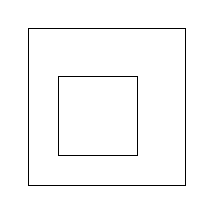
\begin{tikzpicture}
  
   \draw (0,0,1)--(1,0,1)--(1,1,1)--(0,1,1)--cycle;
   \draw (0,0,2)--(2,0,2)--(2,2,2)--(0,2,2)--cycle;
   
    %liquide
    %\draw[fill=white!70!cyan] (0,0) -- ++(6,0) -- ++(0,6) --++ (-6,0) -- cycle;
    %gaz
	%\draw[white, fill=white] (0, 0) -- ++(4.5,0) -- ++(-4.5,4.5) -- cycle;
    %\draw[white,fill=white] (4.5,0) arc (0:90:4.5) ;
    %solute
    %\draw[gray,fill=gray] (0, 0) -- ++(3.5,0) -- ++(-3.5,3.5) -- cycle;
    %\draw[gray, fill=gray, pattern color=black] (3.5,0) arc (0:90:3.5) ;
    %texte
    %\draw (45:6) node {\large liq};
    %\draw (10:4) node {\large gaz};
    %\draw[white] (45:2) node {\large solute};
    %contour
    %\draw[black, thick, fill=none] (0,0) -- ++(6,0) -- ++(0,6) --++ (-6,0) -- cycle;
  \end{tikzpicture}
    \caption{blablabla.}
    \label{fig:Energie libre de binding}
\end{figure}


\subsection{definition}
\subsection{jeux de données}
\subsection{résultats}
